\begin{frame}{\textbf{Parameter Optimization}}

\textbf{Experiment setup}

\begin{itemize}
\item Each posters has corresponded human curated topic in tree structure i.e. 'F.01.r'
\item Assume attendees like one topic
\item One trial, randomly like one poster then compute tree distance between liked poster and first $10$ suggested posters 
\item 'F.01.e' and 'F.01.r' has tree distance 1
\item This distance is used to validate all parameter choices
\end{itemize}

\end{frame}



\begin{frame}{\textbf{Parameter Optimization: number of LSA components}}

\begin{figure}
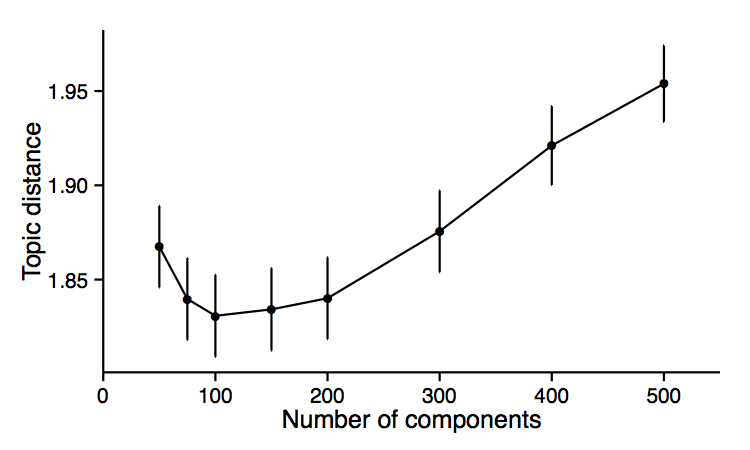
\includegraphics[width=2.2in]{images/performance_vs_components}\\
\tiny{Number of SVD components vs. performance of the algorithm to capture human curated topics}
\end{figure}

Varying SVD components is not significant. Appropriate number of components is around 100.

\end{frame}


\begin{frame}{\textbf{Parameter Optimization: weight for Rocchio algorithm}}

Select one relevant poster and one non-relevant poster (from closest human curated to furthest).

\begin{figure}
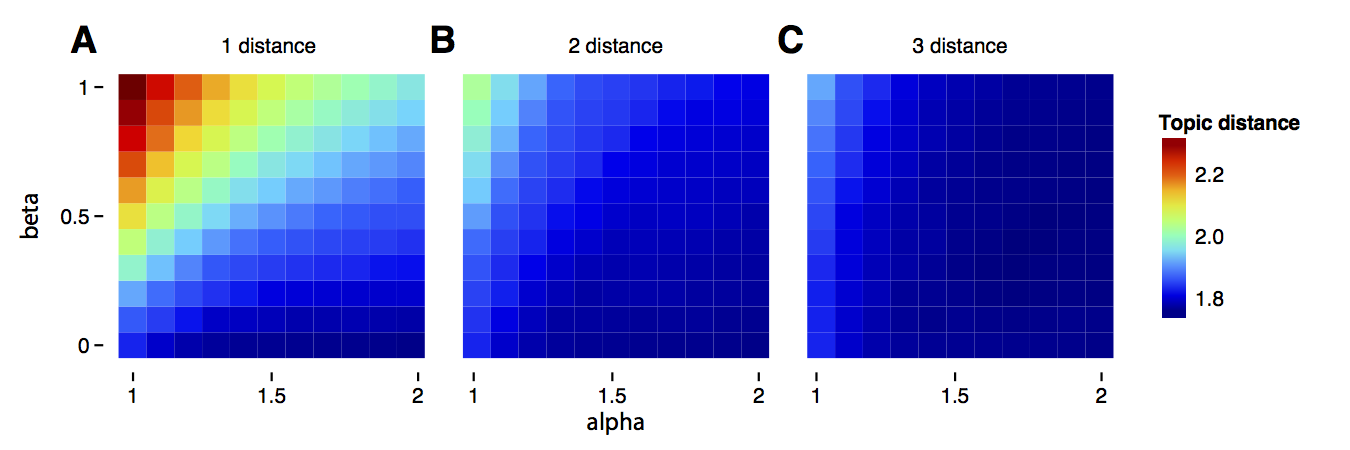
\includegraphics[width=4.0in]{images/alpha_beta_relation_plot}\\
\tiny{Finding best parameters to weigh relevant and non-relevant votes}
\end{figure}

Best combination of parameters for non-relevant posters is $\alpha=1.8$ and $\beta=0$

\end{frame}


\begin{frame}{\textbf{Parameter Optimization: algorithm comparison}}

Effect of more votes on recommendation quality

\begin{figure}
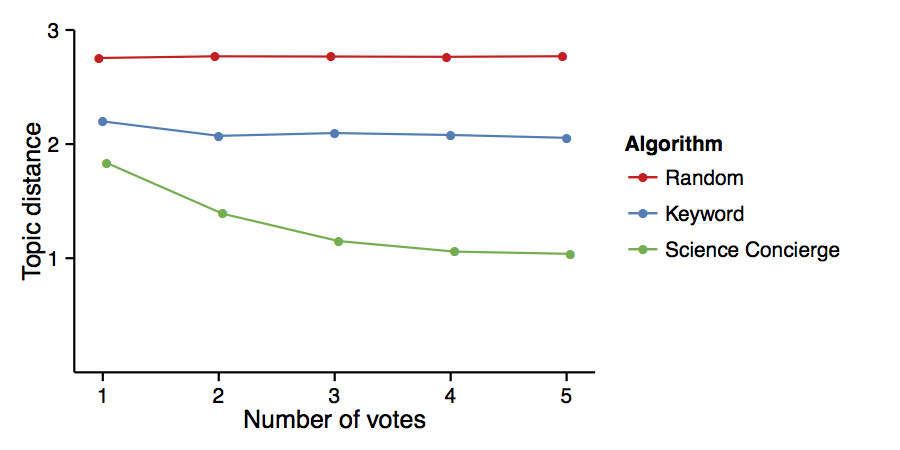
\includegraphics[width=3.0in]{images/performance_vs_votes}\\
\tiny{Comparison of algorithms as they learn more from a simulated user}
\end{figure}


\end{frame}


\begin{frame}{\textbf{Parameter Optimization: algorithm comparison}}

Select two random posters and compute their distance then correlate that difference with human topic distance

\begin{figure}
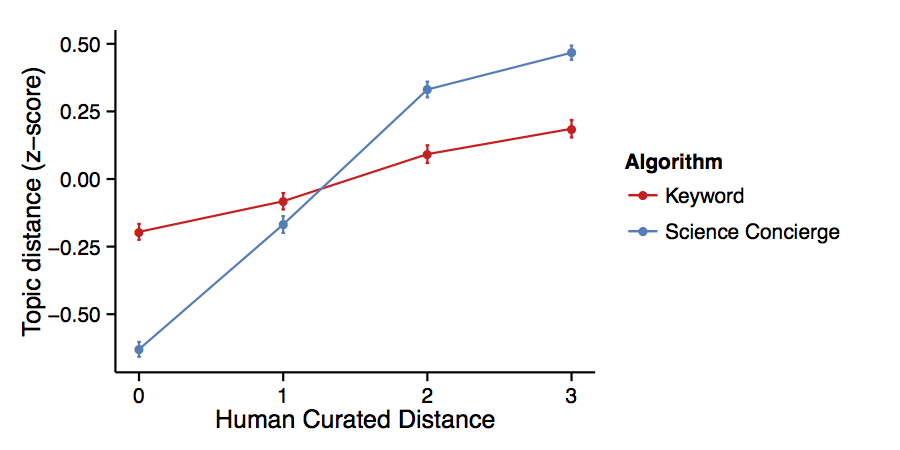
\includegraphics[width=2.5in]{images/human_vs_topic_distance}\\
\tiny{Relationship between human curated distance and topic distance induced by the keyword and Science Concierge models}
\end{figure}

Spearman's rank correlation of the Science Concierge and keywords are $\rho=0.442$, $\rho=0.164$ ($p < 0.001$).

\end{frame}